\chapter{Repository Deep Dive}\label{chap:Repository_Deep_Dive}
In this section, we lightly discuss each of the subdirectories present within the root of Chipyard, take note of any particularly important files, and demonstrate how this entire system is put together.

\section{Makefiles, or the Glue of this Framework}\label{sec:Makefiles_in_Chipyard}
Chipyard makes \textbf{heavy} use of Makefiles to pull together and automate various parts of the build system.
Variables and/or values that are shared between different ways of building systems are higher in the directory structure.

Thus, some of the most overarching commands and variables for this project are defined in \file{chipyard/variables.mk}.
One of the first things defined within this file are numerous output messages.

\subsection{\texttt{SUB\_PROJECT}}\label{subsec:Makefile_SUB_PROJECT}
The first notable part of the \file{variables.mk} file is the \texttt{SUB\_PROJECT} defaulting variable.
This particular variable is what allows for easy re-configuration of the entire framework to support elaborating your own CPU designs.
By changing this file between one of the well-defined options, one can easily re-use major portions of Chipyard's architecture.

For example, to switch from a CPU defined by Chipyard to one that is uses the Hwacha accelerator, one just needs to say \mintinline{bash}{make SUB_PROJCT=hwacha}, and all the necessary configuration variables are changed.

\subsection{Building Each Subproject}\label{subsec:Building_Each_Subproject}
The next notable part of this file is its large \mintinline{make}{ifeq ... endif} blocks.
Each one of these defines a different subproject that can be built and elaborated upon by Chipyard and its surrounding framework.
These subproject defining blocks each define multiple higher-level variables which are the variables that are actually used to build and test each of the CPUs.
Each of the variables is important, and Chipyard provided documentation for each variable inside \file{variables.mk}.
However, additional information that we gathered through trial-and-error is presented below.

\begin{description}
\item[\texttt{SUB\_PROJECT}] This corresponds to one of the projects in the \file{chipyard/generators} directory.
  More formally, it is defined by one of the entries in the \file{build.sbt} files in the respective generators directory, and by the main \file{build.sbt} file in the root of Chipyard.
\item[\texttt{SBT\_PROJECT}] This corresponds to a top-level of the repository of the chip to build.
  This is where many of the higher-level constructs, such as the test harness and test bench are defined from.
\item[\texttt{MODEL}] The model is the top-level module of the project that should be used by Chisel.
  Normally, this should be defined to the be same as the test harness, but does not necessarily have to be.
\item[\texttt{VLOG\_MODEL}] This is the top-level module of the project that should be used by FIRRTL/Verilog.
  Like \texttt{MODEL}, this is usually the same as the test harness, but does not necessarily need to be.
\item[\texttt{MODEL\_PACKAGE}] This is the Scala package that is used to find the overall model of the CPU.\@
  This should correspond to the \mintinline{scala}{package <packageName>} in a Scala CPU configuration file.
\item[\texttt{CONFIG}] This defines the parameters that should be used for the project.
  Typically, this is used to select one of the CPU configurations defined in the \texttt{SBT\_PROJECT}.
\item[\texttt{CONFIG\_PACKAGE}] This is the Scala package that defines the \texttt{Config} class.
  This file \textbf{MUST} contain the class definition for \texttt{Config}, meaning \mintinline{scala}{object Config} must be present.
\item[\texttt{GENERATOR\_PACKAGE}] This is the Scala package that defines the \texttt{Generator} class.
  This file \textbf{MUST} contain the class definition for \texttt{Generator}, meaning \mintinline{scala}{object Generator} must be present.
\item[\texttt{TB}] This defines the test bench wrapper that extends over the test harness to allow for simulation in a Verilog simulator.
\item[\texttt{TOP}] This is the top-level module of the project.
  Typically, this is the module instantiated by the test harness.
\end{description}

\section{\file{build.sbt}}\label{sec:build.sbt}
There are two main \file{build.sbt} files that you should be aware of.
There is a \file{build.sbt} for each of the generator subdirectories.
These define some metadata information about each of the projects, such as the name of the design, the authors of the design, the targeted \texttt{sbt} version, and others.

However, the \file{build.sbt} file in the root of Chipyard is a metadata file not just for Chipyard itself, but also pulls together all the dependencies in \file{chipyard/generators/} so that they all can be elaborated upon with Chipyard.

% TODO: Rework this paragraph about circular dependency in main build.sbt file.
This file is also the one that should be used for defining your \emph{own} CPU.\@
Note that this means you are building your own Verilog code which defines the generation rules for a CPU.\@
However, one must be careful that they do not introduce circular dependencies into the dependency graph between the CPU generation and elaboration tools.
Even though Scala has support for lazy evaluation, it does not completely extend to dependency evaluation, and the entire system can fall apart.
This does \emph{not} mean that you use this to build a new CPU on top of the architecture already defined by Chipyard, or any other CPU.\@
However, you can use other CPU-generating systems inside your design.

\subsection{About}\label{sec:About_Verilator_Simulator}
The primary way to simulate SoCs' designed using the Chipyard framework is via Verilator simulations.
The directory for verilator is \file{chipyard/sims/verilator}.
An example simulation can be run by using \mintinline{bash}{make} in the verilator directory.
Running the \texttt{make} command produces a simulator executable in the verilator directory.

Custom Chipyard configs can be simulated by running \mintinline{bash}{make CONFIG=<your custom config>}.
For example, if your project name was ``TestConfig'', running \mintinline{bash}{make CONFIG=TestConfig} would create an executable called \file{simulator-chipyard-TestConfig} in the \file{verilator} directory.
Custom RISCV code can be run by using the command \mintinline{bash}{./simulator-chipyard-TestConfig /path/to/riscv/executable} from the \file{chipyard/sims/verilator} directory.

\section{Generators}\label{sec:Generators}
In this section, we look at each of the subdirectories inside the \file{chipyard/generators} subdirectory in turn.
Each of the CPU generators presented below are each slightly unique in their implementation of the open RISC-V ISA.\@

\subsection{BOOM}\label{sec:BOOM_Generator}
\nocite{boomHomepage}
BOOM~(Berkeley Out-of-Order Machine) is a CPU defined and built by Univerity of California at Berkeley that implements the RISC-V Instruction Set Architecture (ISA).
Its claim to fame is that it can execute RISC-V instructions out-of-order, thereby drastically improving performance.
It is designed to be highly performant, synthesizable, and parameterizable.

BOOM includes support for the following operations:
\begin{itemize}
\item Floating Point (IEEE 754--2008)
\item Atomic Operations
\item Caching
\item Virtual Memory
\end{itemize}
In addition, BOOM supports external debugging.
Microarchitectural documentation can be found \href{https://docs.boom-core.org/en/latest/}{here}.
The GitHub organization and its development can be found \href{https://github.com/riscv-boom}{here}.

These CPU definitions are used by \nameref{sec:Chipyard_Generator} when elaborating CPU designs defined by the end-programmer.

\subsection{Chipyard}\label{sec:Chipyard_Generator}
This is the main source of truth inside this repository.
Here is where all of the code required to get these disparate CPUs to work and build together is located.
Typically, very little editing is needed to be done here.
Most of the editing in this repository comes in the form of defining your own CPUs, which are themselves defined in terms of other CPUs or other lower-level Chipyard constructs.

\subsection{cva6}\label{sec:cva6_Generator}
\nocite{cva6Github}
\nocite{zaruba2019cost}
cva6 is a 6-stage, single issue, in-order CPU.\@
This means that unlike the \nameref{sec:BOOM_Generator} design, instructions are \emph{always} executed in order.

\subsubsection{Gemmini}\label{sec:Gemmini_Generator}
\subsubsection{Hwacha}\label{sec:Hwacha}
\subsubsection{Icenet}\label{sec:Icenet_Generator}
\subsubsection{NVDLA}\label{sec:NVDLA_Generator}
\subsubsection{RISC-V Sodor}\label{sec:RISC-V_Sodor}
\subsubsection{Rocket-Chip}\label{sec:Rocket_Chip}
\subsubsection{SHA3}\label{sec:SHA3_Accelerators_Generator}
\subsubsection{SiFive Blocks}\label{sec:SiFive_Blocks}
\subsubsection{SiFive Cache}\label{sec:SiFive_Cache}
\subsubsection{\file{testchipip}}\label{sec:testchipip}

\section{Custom Configurations}\label{sec:Custom_Configurations}
Custom Configs can be created in the directory \mintinline{bash}{chipyard/generators/chipyard/src/main/scala/config/}.
For example, I created a new scala file called \file{NewTestConfig.scala} in the directory, allowing me to create a simulator from a class inside the NewTestConfig.scala file.
Example Configs can be found in  \file{RocketConfigs.scala} in the same directory.

% TODO: Include custom config example

\section{Verilator Simulator}\label{sec:Verilator_Simulator}

\subsection{FPGA Implementation}\label{sec:FPGA_Implementation}


\subsubsection{About}\label{sec:About}

\begin{figure}[h!tbp]
  \centering
  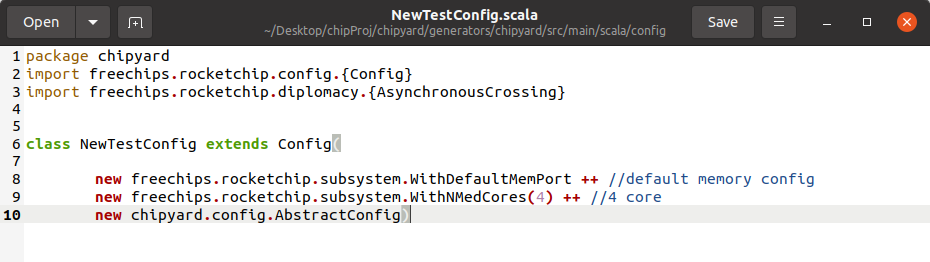
\includegraphics[width=0.7\linewidth]{./NewTestConfig.png}
  \caption{\file{NewTestConfig.scala}}
  \label{fig:newtestconfig}
\end{figure}

%%% Local Variables:
%%% mode: latex
%%% TeX-master: "../doc"
%%% End:
